\documentclass[ps1.tex]{subfiles}
%\usepackage{enumerate}
%\usepackage[left=3cm,right=3cm,bottom=3cm,top=2cm]{geometry}
\begin{document}
\section* {(15 points) Double-slit interference of electrons}

\begin{enumerate}[(a)]
\item Electrons of momentum p fall normally on a pair of slits separated by a distance d. What is the distance, w, between adjacent maxima of the interference fringe pattern formed on a screen a distance D beyond the slits? note: You may assume that the width of the slits is much less than the electron de Broglie wavelength.

\item In an experiment performed by Jonsson in 1961(!!!), electrons were accelerated through a 50kV potential towards two slits separated by a distance $d = 2\cdot10^{-4}$ cm, then detected on a screen D = 35 cm beyond the slits. Calculate the electron's de Broglie wavelength, $\lambda$, and the fringe spacing, w.
\item What values would d, D, and w take if Jonsson?s apparatus were simply scaled up for use with visible light rather than electrons?
\end{enumerate}

\noindent\makebox[\linewidth]{\rule{\paperwidth}{0.4pt}}

\begin{enumerate}[(a)]
\item \begin{figure}[ht!]
\centering
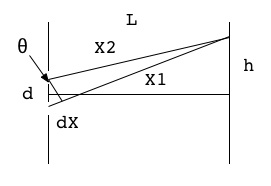
\includegraphics[width=55mm]{img/slit_diagram.jpg}
\caption{Double Slit Geometry}
\label{overflow}
\end{figure}
\noindent
$\Delta x = x_2 - x_1 = m\lambda$ when $m = 0, 1, 2, \dots$

$\theta = sin(\frac {m\lambda}{d}) = \frac {m\lambda}{d}$

$H = Lsin(\theta) \approx L\theta = \frac {m\lambda L}{d}$
$ w = H_{m+1} - H_m = (m+1)\frac {\lambda L}{d} - m\frac {\lambda L}{d} = \frac {\lambda L}{d}$

for an electron $\lambda = \frac {h}{p}$ so $w = \frac {hL}{pd}$\\

\noindent\makebox[\linewidth]{\rule{\paperwidth}{0.4pt}}
\item $v = \sqrt(\frac {2e\Delta V}{m}) = \sqrt(\frac {2(1.6\cdot10^{-19}(50)}{9.11\cdot10^{-31}}) = 4.19\cdot10^6$

de Broglie Wavelength $\lambda = \frac {h} {p} = \frac {h}{mv} = \frac {6.63\cdot10^{-34}}{(9.11\cdot10^{-31})(4.19\cdot10^6} = 1.74\cdot10^{-10}$

$w = \frac {hL}{pd} = \frac {(6.63\cdot10^{-34}) 0.35} {(9.11\cdot10^{-31})(4.19\cdot10^6)(2\cdot10^{-7})} = 3.04\cdot10^{-4}$

\noindent\makebox[\linewidth]{\rule{\paperwidth}{0.4pt}}
\item Not sure whats being asked for here.  there are three unknowns with only one equation

\end {enumerate}
\noindent\makebox[\linewidth]{\rule{\paperwidth}{0.4pt}}

\end{document}